% 한글본. lualatex 로 컴파일한다 (fontspec + Noto Sans KR). 영문본과 같은 그림·표 자료를 쓴다.
\documentclass[final,5p,times,twocolumn]{elsarticle}

\usepackage{fontspec}
\setmainfont{Noto Sans KR}
\setsansfont{Noto Sans KR}
\usepackage{amsmath,amssymb}
\usepackage{booktabs}
\usepackage{multirow}
\usepackage{xcolor}
\usepackage{graphicx}
\usepackage{url}
\usepackage[hidelinks]{hyperref}
\graphicspath{{../../figures/}}
\renewcommand{\figurename}{그림}
\renewcommand{\tablename}{표}

% TODO: 투고 저널은 저자가 정한다
\journal{Transportation Research Part C: Emerging Technologies}

\newcommand{\pending}[1]{\textcolor{red}{[#1]}}

\begin{document}

\begin{frontmatter}

\title{연결성 제약 드론 배송을 위한 기하 및 학습 기반 중계 제어}

\author[ku]{고광종}
\ead{koptimizer@korea.ac.kr}
\author[ku]{정태수\corref{cor1}}
\ead{tcheong@korea.ac.kr}
\cortext[cor1]{교신저자.}
\affiliation[ku]{organization={고려대학교 산업경영공학부},
                 addressline={서울특별시 성북구 안암로 145},
                 city={서울},
                 postcode={02841},
                 country={대한민국}}

\begin{abstract}
재난 구호에서 배송 드론은 편대 스스로 구성하는 다중 홉 중계 사슬을 통해 제어 센터와 연결을 유지한
채, 제한된 적재량으로 물자를 나르고 재적재를 위해 복귀해야 한다. 본 연구는 이를 모든 드론이 배송과
중계를 겸할 수 있고 연결성이 매 스텝 강제되는 makespan 최소화 문제로 모형화한다. 같은
연결성 보존 투영을 공유하는 두 제어기를 제안한다. 교착 탈출 장치를 갖춘 기하 사슬 중계 휴리스틱과,
집합 기반 자기회귀 상위 정책을 이산 soft actor-critic 으로 한 번 학습한 편대 크기 불변 정책이다.
두 제어기를 드론 3--10대, 목적지 20--300곳의 동일 인스턴스에서 쌍별로 비교하고, 무학습 베이스라인
넷과 작은 인스턴스의 시간 확장 혼합정수 참조 모형에 대조한다. 학습 정책은 모든 구성의 모든
인스턴스를 완주하고, 휴리스틱은 탈출 장치가 있을 때 98--100\%, 없을 때 62\%를 완주한다. 두 제어기는
구성 공간을 나눈다. 드론 3대에서는 휴리스틱이 쌍별 중앙값으로 30--39스텝 빠르고, 4대에서는 480
롤아웃에서 동률이며, 5대 이상에서는 학습 정책이 38--178스텝 빠르고 그 격차는 편대가 커질수록
커진다. 3대 구성의 열세는 어느 드론이 중계할지라는 한 결정에 국소화되며, 정보·크레딧 할당·결정
구조·초기화·보상 설계에 걸친 정책 쪽 개입 열 가지가 모두 이를 제거하지 못한다. 연결성 투영을 같은
방향 축소에서 접선 보존으로 바꾸면 열세의 절반이 사라져, 이 열세가 학습기만이 아니라 제약을
강제하는 방식의 성질이기도 함을 보인다. 두 제어기 모두 결정당 밀리초에 동작하며, 이는 목적지 10곳에서
90분 안에 계획을 내지 못하는 정확 최적화보다 세 자릿수 빠르다.
\end{abstract}

\begin{keyword}
드론 배송 \sep 중계 네트워크 \sep 연결성 제약 \sep 다중 에이전트 강화학습 \sep 휴리스틱 \sep
재난 물류
\end{keyword}

\end{frontmatter}

% =====================================================================================
\section{서론}
\label{sec:intro}

통신·물류·도로 기반이 파괴되면 드론 편대가 임시 제어 센터에서 여러 목적지로 긴급 물자를 나를 수
있다. 이것이 택배 배송과 다른 점은 둘이다. 첫째, 상·하역이 원격으로 감독되고 배송 상태가 추적되어야
하므로 모든 드론이 항상 제어 센터와 통신 가능해야 하며, 지상망이 사라진 상황에서 그 통신은 드론들이
스스로 다중 홉 사슬의 중계 노드가 되어야만 성립한다. 둘째, 편대는 작고 드론 한 대의 적재량은 몇
단위에 불과해 드론은 센터와 목적지 사이를 왕복하며, 중계로 서 있는 드론은 그만큼 배송하지 않는
드론이다. 따라서 운영상의 질문은, 사슬을 한 번도 끊지 않으면서 마지막 목적지를 가능한 한 빨리
배송하도록 배송 역할과 중계 역할을 시간에 따라 어떻게 배정하느냐다.

이 문제가 어려운 이유는 세 가지다. 하드 연결성 제약은 교착을 만든다. 모든 드론을 가장 가까운
목적지로 보내는 탐욕 배정은 본 연구의 표준 인스턴스를 한 건도 완주하지 못하는데, 편대가 스스로를
잡아당기다가 어떤 드론도 움직일 수 없게 되기 때문이다. 중계는 처리량과 직접 경쟁하므로 적정한 중계
대수와 중계 드론은 남은 목적지의 기하와 적재가 남은 드론 수에 따라 달라진다. 그리고 정확 최적화는
규모가 커지지 않는다. 98 m 격자 위의 시간 확장 혼합정수 모형은 목적지 4곳과 6곳의 계획은 내지만
10곳에서는 90분 안에 실행 가능한 계획을 찾지 못한다.

\paragraph{제안}
이 문제에 대해 두 제어기를 제안하고 나란히 연구한다.
\begin{enumerate}
\item \emph{기하 사슬 중계 휴리스틱}. 적재가 남은 드론 중 센터에서 가장 먼 드론이 선두이고,
중계 대수는 선두의 목표가 필요로 하는 통신 홉 수이며, 중계 드론은 그 다음으로 먼 드론들로서 센터에서
선두까지의 선분 위에 $0.9R$ 간격으로 선다. 규칙이 결정론적이라 교착된 배정을 무한히 반복할 수
있으므로, 편대가 정해진 스텝 수만큼 정체하면 선두를 교대하는 \emph{교착 탈출} 장치를 더했다. 탈출
장치만으로 표준 구성 완주율이 62\%에서 98\%로 오른다.
\item 편대 크기에 불변인 \emph{학습 정책}. 상위 정책이 20스텝마다 드론별로 일곱 개 이산 옵션
중 하나를 배정한다. 드론·후보 목적지·중계 슬롯을 집합으로 부호화하고 어텐션으로 풀링하며,
선두 하나와 중계 $k$대의 대형을 의도적으로 구성할 수 있도록 자기회귀로 결정한다. 드론 3·4대 편대로
이산 soft actor-critic 으로 한 번 학습한 뒤 재학습 없이 최대 10대 편대에서 돌린다.
\end{enumerate}
두 제어기 모두 같은 연결성 보존 투영을 거쳐 행동한다. 명령된 이동은 편대의 연결이 유지되는 최대
비율로 축소된다. 따라서 연결성은 두 제어기 모두에 구조적으로 보장되며, 실험의 질문은 제약을
위반하는가가 아니라 제약 아래에서 진척을 내는가다.

\paragraph{연구 질문}
연구를 네 질문으로 조직한다.
\begin{itemize}
\item[\textbf{RQ1}] 제안 제어기들은 매 스텝 연결성이 강제된 채 항상 완주하는가, 못 한다면 왜인가?
\item[\textbf{RQ2}] 작은 인스턴스에서 제안 제어기들은 격자 모형의 정확 최적화로 얻은 참조 계획에
얼마나 가까운가?
\item[\textbf{RQ3}] 두 제어기의 성능은 편대 크기·목적지 수·거점 위치·통신 반경에 따라 어떻게
다르고, 그 차이는 어디서 오는가?
\item[\textbf{RQ4}] 각 제어기의 구성 요소는 필수적인가?
\end{itemize}

\paragraph{발견}
학습 정책은 시험한 모든 구성의 모든 인스턴스를 완주하고, 휴리스틱은 탈출 장치와 함께
98--100\%를 완주한다(RQ1). 격자 모형이 다룰 만큼 작은 인스턴스에서 두 제어기는 참조 계획의 수
퍼센트 안에 있고, 참조 계획 자체는 연속 문제의 하한이 아니라 제한이다(RQ2). 두 제어기는 편대
크기로 구성 공간을 나눈다. 3대에서는 휴리스틱이 빠르고, 4대에서는 동률이며, 5대 이상에서는 학습
정책이 빠르고 10대에서 격차가 178스텝까지 커진다. 3대 열세는 어느 드론이 중계할지라는 한 결정이며
정책 쪽 개입 열 가지에 저항하지만 연결성 투영을 바꾸면 절반으로 줄어든다(RQ3). 학습 정책에서 규칙
정규화·구성 무작위화·엔트로피 감쇠를 빼면 수백 스텝 또는 완주를 잃고, 휴리스틱에서 탈출 장치를
빼면 완주의 3분의 1을 잃는다(RQ4).

\paragraph{기여}
(i) 제약이 구조적으로 성립하는 투영 위에 세운, 교착 탈출을 갖춘 기하 사슬 중계 휴리스틱과 편대 크기
불변 학습 정책. (ii) 두 제어기가 상보적임을 보이는 편대 크기별 쌍별 평가와 그 경계의 기제.
(iii) 학습기를 바꿔 드론 부족 영역의 열세를 좁히려는 열 가지 기록된 음성 결과와, 열세의 절반이
강제 모형에 귀속됨을 보이는 민감도 결과. (iv) 무엇을 제한하고 무엇을 제한하지 못하는지를 정직하게
밝힌 격자 MILP 참조.

% =====================================================================================
\section{관련 연구}
\label{sec:related}

\paragraph{드론 배송 경로}
드론을 이용한 경로 문제는 flying-sidekick 외판원 문제 \cite{murray2015}와 그 다중 드론 확장
\cite{murray2020,agatz2018,dorling2017} 이래 연구되어 왔다. 이 모형들은 통신을 공짜로 본다. 드론이
도달 가능해야 한다는 요구가 없고, 어떤 차량도 중계를 위해 배송 역할을 내려놓지 않는다. min-max
다중 차량 경로의 학습 해법 \cite{park2023,guo2024}은 집합 기반 정책이 문제 크기에 걸쳐 일반화함을
보이는데, 이는 편대 크기에 걸쳐 우리가 필요로 하는 성질이지만 역시 연결성 제약이 없다. 같은 드론이
배송과 감지를 겸하는 이중 임무 편대 \cite{zhu2026}는 배송당 우회 예산을 정식화하지만 부차 임무가
통신이 아니라 감지다.

\paragraph{UAV 중계와 연결성 유지}
공중 중계 배치는 자체 문헌을 이루며 \cite{zeng2016,yanmaz2022,ding2022}, 임무 UAV와 중계 UAV를
다중 에이전트 학습으로 공동 최적화하는 연구도 있다 \cite{mutto2024,maen2024}. 이 연구들에서 중계는
임무 그 자체이거나 자체 보상을 가진 전용 하위 편대이며, 적재도 재적재도 없고 배송 makespan 을
최소화하지 않는다. 다중 로봇 항법의 연결성 유지는 학습 제어기로 접근된 바 있다 \cite{li2021}.
임무 역할과 중계 역할 사이의 전환은 다중 로봇 탐사 \cite{dehoog2009,cesare2015}에서 확립된
아이디어로, 중계 로봇이 착륙해 고정 노드가 된다.

\paragraph{본 연구의 위치}
저자들이 아는 범위에서 (i) 적재와 재적재가 있는 동질 편대가 물리적 화물을 다수 목적지로 나르고,
(ii) 모든 드론이 매 스텝 다중 홉 사슬로 센터에 연결되어야 하며, (iii) makespan 을 목적으로 하는
설정을 함께 다룬 연구는 없다. 이 설정에서는 중계 의무가 화물 처리량과 경쟁하고 편대가 거점으로
반복 복귀해야 하므로, 역할 배정이 일회성 배치가 아니라 순차 결정이 된다.

\paragraph{학습 기법}
학습 측면에서는 soft actor-critic \cite{haarnoja2018}, 분산 실행을 위한 중앙 critic
\cite{lowe2017,foerster2018}, 가치 분해 \cite{sunehag2018,rashid2018}, 반 마르코프 결정 과정으로서의
옵션 \cite{sutton1999}, 무효 행동 마스킹 \cite{huang2022}, 안전 행동 투영 \cite{dalal2018}에
기반한다. \ref{sec:negative}절의 음성 결과는 이 아이디어 중 여럿을 직접 시험한다. 드론별 크레딧,
결합 행동 critic, 단조 가치 혼합, 잠재 함수형 보상 설계 \cite{ng1999}를 드론 부족 영역의 열세에
대한 처방으로 시도했고 어느 것도 열세를 제거하지 못했다.

% =====================================================================================
\section{문제 정의}
\label{sec:problem}

제어 센터는 $c \in [0,1000]^2$ m에 있고 $M$개 목적지 $d_1,\dots,d_M$는 센터로부터 $0.9\,N R$
안에 놓인다. $N$은 드론 수, $R = 300$\,m는 통신 반경이다. 각 드론은 $v = 13.89$\,m/s로 비행하고
$Q = 5$단위를 싣고, 목적지에서 $S = 10$스텝에 한 단위를 내리며 센터에서 $S$스텝에 $Q$까지
재적재한다. 목적지나 센터는 25\,m 안에 들어오면 도달한 것으로 보며 한 스텝은 1초다. 모든 목적지는
정확히 한 단위를 필요로 한다. 드론 간 충돌·바람·배터리는 모형화하지 않는다.

\paragraph{연결성}
$G_t$를 센터와 $N$대 드론을 정점으로, 서로 $R$ 안에 있는 정점 쌍을 간선으로 하는 그래프라 하자.
$G_t$가 연결되어 있으면 스텝 $t$에 편대가 \emph{연결}된 것이고, 이는 모든 드론이 센터까지 다중 홉
경로를 가진다는 말과 같다. 제약은 모든 $t$에서 $G_t$가 연결되는 것이며, 벌점이 아니라 강제로
지킨다(\ref{sec:projection}절).

\paragraph{목적}
makespan 은 마지막 목적지가 배송되는 스텝이다. 제어기가 10{,}000스텝 예산 안에 모든 목적지를
배송하면 그 인스턴스를 \emph{완주}한 것으로 본다. 완주율과, 완주한 인스턴스에서의 makespan 을
보고한다.

\paragraph{구성}
구성은 편대 크기 $N$, 목적지 수 $M$, 거점 배치(지도 중앙 고정 또는 균일 무작위)의 세 쌍이다.
\emph{표준} 구성은 고정 거점의 $N=4$, $M=50$이다. 학습 정책은 $N \in \{3,4\}$, $M \in [20,80]$,
무작위 거점으로 학습하며 그 외 구성은 본 적이 없다. 휴리스틱에는 학습이 없다.

% =====================================================================================
\section{제안 제어기}
\label{sec:method}

그림~\ref{fig:overview}에 설정과 두 제어기를 요약했다. 두 제어기는 \emph{목표} 수준에서
결정한다. 매 결정 시점에 각 드론은 목표(목적지, 센터, 또는 중계 슬롯)를 받고 그곳으로 전속
직진한다. 결정은 20스텝마다, 또는 목표가 무효해지는 즉시(다른 드론이 그 목적지를 배송했거나,
적재가 떨어졌거나, 사슬이 짧아져 중계 슬롯이 사라졌을 때) 갱신한다. 옵션 집합은 둘이 같다. 후보
목적지 다섯 곳(가장 가까운 미배송 세 곳과 센터에서 가장 먼 두 곳), 센터 복귀, 중계. 중계 슬롯은
센터에서 선두 드론까지의 선분 위 $0.9R$의 배수 지점에 놓이고 환경이 배정하므로, 제어기는 중계할지
\emph{여부}만 결정한다.

\begin{figure*}[t]
\centering
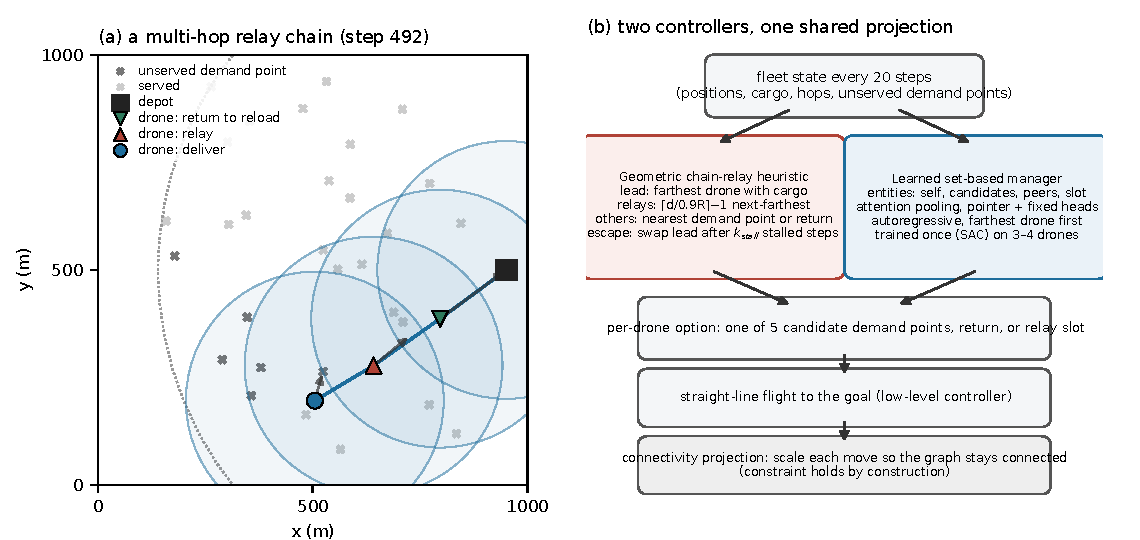
\includegraphics[width=\linewidth]{fig_overview_v5_26_10_17_15.pdf}
\caption{(a) 드론 3대 인스턴스에서 휴리스틱으로 220스텝 진행한 상태. 선두 드론(파란 원)이 먼
목적지로 향하고, 한 대가 센터까지의 선분 위에서 중계하며(빨간 삼각형), 한 대는 재적재를 위해
복귀한다. 음영 원판은 통신 반경, 점선 원은 도달 영역 $0.9NR$이다. (b) 두 제어기는 같은 드론별
옵션을 내고 직진 하위 제어기와 연결성 투영을 공유한다.}
\label{fig:overview}
\end{figure*}

\subsection{연결성 보존 투영}
\label{sec:projection}

단절에 대한 보상 벌점은 어떤 행동으로도 막을 수 없는 상황을 벌한다. 예컨대 하역 중 정지한 드론은
동료가 떠나면 고립된다. 따라서 제약을 투영으로 강제한다. 모든 드론의 명령 변위가 주어지면, 투영은
드론 하나씩 편대가 연결을 유지하는 $[0,1]$ 안의 최대 배율을 찾는다. 매 회차 제한했을 때 연결된
드론이 가장 많이 남는 드론을 고르고, 특정 앵커 드론이 굶지 않도록 동점은 무작위로 깬다. 변위가
10\% 아래로 축소된 드론은 그 스텝에 \emph{정체}한 것으로 센다. 직전 위치는 항상 연결 상태이므로
배율 0은 유효한 대안이고 제약은 구조적으로 성립한다. 변위가 방향을 유지한 채 크기만 잃으므로 이를
\emph{같은 방향} 투영이라 부른다. \ref{sec:sensitivity}절에서 접선 성분을 남기는 대안을 다룬다.

\subsection{교착 탈출을 갖춘 기하 사슬 중계 휴리스틱}
\label{sec:heuristic}

\paragraph{배정 규칙}
$r_i$를 드론 $i$의 센터 거리라 하자. \emph{선두}는 적재가 있는 드론 중 센터에서 가장 먼 드론이다.
선두의 목표는 가장 가까운 미배송 목적지이며 센터로부터 거리 $d$에 있다. 사슬에는
$h = \lceil d / (0.9R) \rceil$ 홉, 즉 $h - 1$대의 중계가 필요하고 이는 $N-1$을 넘지 않는다. 선두가
아닌 드론 중 센터에서 가장 먼 $h-1$대를 중계로 배정하고, 적재가 있는 나머지 드론은 가장 가까운
미배송 목적지로, 적재가 없는 드론은 센터로 보낸다. 규칙은 매 결정 시점에 평가되며 비용은
$O(N \log N)$이다.

\paragraph{교착 탈출}
규칙은 결정론적이라 어떤 기하가 편대를 정체시키면 같은 배정을 다시 내고 정체가 지속된다. 탈출
장치가 없으면 규칙은 표준 인스턴스의 62\%만 완주한다. 이동을 시도한 드론 중 최대 한 대를 뺀
나머지가 투영에 막혔을 때 \emph{부분 교착}으로 본다. 부분 교착이 $k_{\mathrm{stall}}$스텝 지속되면
$h_{\mathrm{hold}}$스텝 동안 탈출 단계에 들어가, 적재가 있는 다음으로 먼 드론이 선두가 되고 원래
선두는 센터로 복귀한다. 한 에피소드의 $n$번째 탈출에서는 $n$번째로 먼 드론이 선두가 되어 반복
탈출이 편대를 순환한다. 선두를 제외한 전원이 센터 쪽으로 물러나 사슬을 느슨하게 하는 대안 모드도
구현했다. $k_{\mathrm{stall}} = 120$, $h_{\mathrm{hold}} = 20$, 선두 교대 모드는
\ref{sec:rq4-heuristic}절에서 평가 시드와 분리된 시드로 골랐으며, 본 논문의 모든 비교에 이 설정을
쓴다.

\subsection{편대 크기 불변 학습 정책}
\label{sec:learned}

\paragraph{결정 구조}
학습 제어기는 매 결정 시점에 드론마다 $K = 7$개 옵션 중 하나를 내는 상위 정책이고, 하위 제어기는
휴리스틱과 같은 직진 비행이다. 초기 버전에서 학습 하위 제어기를 시도했으나 완주율을 0--2\%로 떨어뜨려
쓰지 않는다. 결정 시점 사이에서 환경은 반 마르코프 결정 과정 \cite{sutton1999}이며 상위 정책의
전이는 옵션의 할인 수익을 저장한다.

\paragraph{집합 기반 인코더}
각 드론은 네 종류의 엔티티로 부호화된다. 자기 상태(10개 특징: 적재, 센터 거리, 홉 깊이, 미배송
비율, 시각, 이동 비율, 정체 지표, 서비스 타이머, 절단점 지표), 후보 목적지 다섯(각 6개 특징:
거리, 방향, 동료가 이미 겨냥했는지, 센터 거리, 필요 홉 수), 동료($N-1$개 엔티티, 각 9개 특징: 상대
위치, 적재, 홉 깊이, 동료 현재 역할의 원핫), 중계 슬롯(4개 특징). 거리는 지도 크기가 아니라 $R$로
정규화한다. 엔티티 종류별로 폭 128의 2층 MLP를 통과시키고, 자기 임베딩을 질의로 두 다중 헤드
어텐션 층이 동료 집합과 후보 집합을 풀링하며, 네 벡터를 이어 붙여 융합한다. 포인터 헤드가 융합
임베딩에 대해 후보 다섯을 점수 매기고 고정 헤드가 \emph{복귀}와 \emph{중계}를 점수 매긴다.
네트워크 어디에도 $N$이나 $M$에 의존하는 것이 없어 한 가중치가 본 적 없는 편대에서 돈다. 무효
옵션은 마스크한다 \cite{huang2022}.

\paragraph{자기회귀 결정}
드론을 센터 거리 내림차순으로 정렬해 먼 드론부터 결정하고, 각 드론의 옵션이 표본된 뒤 그 새
역할을 이후 드론들이 보는 동료 특징에 써넣는다. 선두 하나와 중계 $k$대의 대형은 드론별 독립
표본으로는 우연히만 나오지만 순차 결정에서는 의도적으로 구성할 수 있다. 대가는 결정 1회에 $N$번의
순차 네트워크 호출이다.

\paragraph{학습}
상위 정책은 이산 soft actor-critic \cite{haarnoja2018}으로 학습한다. 드론 임베딩 사이에 어텐션을
둔 twin-Q critic이 드론별 행동가치를 내고 그 드론 평균을 팀 수익에 회귀하며, actor 손실은 표준
기대값 형태다. 팀 보상은 배송당 $+10$, 재적재당 $+30$, 스텝당 $-0.01N$, 미배송 비율에 비례하는
잔여 벌점 $-0.1N$이고 할인율은 스텝당 $\gamma = 0.997$이다. 세 요소가 중요하다. (i) \emph{엔트로피
목표 감쇠}: 관행적 목표 $0.6\log n_{\mathrm{valid}}$는 정책을 너무 무작위하게 유지해 여러 스텝의
대형을 지키지 못하게 하는데, 그 무작위성은 동시에 교착된 편대가 탈출하는 유일한 수단이기도 하다.
목표를 처음 400 에피소드 동안 $0.6\log n$에서 $0.25\log n$으로 선형 감쇠시키자 표준 구성 makespan
이 1{,}418에서 900대로 내려갔다. (ii) \emph{규칙 정규화}: 가중치 2.0의 교차엔트로피 항이 휴리스틱
배정 규칙이 택할 행동 쪽으로 정책을 당긴다(그 행동이 마스크되지 않은 경우에 한해).
(iii) \emph{구성 무작위화}: $N$, $M$, 거점을 에피소드마다 다시 뽑는다. 최적화는 Adam
$3\times10^{-4}$, 재생 버퍼 60{,}000에서 옵션 전이 256개 배치, $\tau = 0.005$의 Polyak 평균을
쓴다. 체크포인트는 50 에피소드마다 3{,}000스텝 예산의 홀드아웃 80개에서 $100f + 40(1 - \bar
t/3000)$으로 고른다($f$는 완주율, $\bar t$는 평균 스텝으로 완주 1퍼센트포인트가 75스텝 값어치다).
학습은 8회 연속 갱신이 없거나 1{,}000 에피소드에서 멈춘다. RTX~5080 하나를 네 실행이 나눠 쓸 때 한
실행에 약 13시간이 든다.

% =====================================================================================
\section{실험 설계}
\label{sec:setup}

\paragraph{인스턴스와 구성}
인스턴스는 정수 시드로 생성되며 시드·$N$·$M$·거점 모드가 인스턴스를 정확히 결정하므로 두 제어기를
동일 인스턴스에서 돌릴 수 있다. 평가 시드는 학습·체크포인트 선택·휴리스틱 튜닝에 쓴 시드와 겹치지
않는다. 표준 구성($N=4$, $M=50$, 고정 거점)과 무작위 거점의 미지 구성 일곱 개
$N/M \in \{3/20, 3/30, 4/80, 5/50, 6/80, 8/150, 10/300\}$에서 평가한다.

\paragraph{베이스라인}
두 제안 제어기 외에 중계 없는 탐욕 배정, 한 대 또는 두 대를 영구 중계로 두는 고정 중계 정책 둘,
그리고 탈출 장치 없는 기하 규칙을 돌린다. 이들은 문제가 단순 배정으로 풀리지 않음을 보인다.

\paragraph{참조 모형}
작은 인스턴스는 Gurobi~13 \cite{gurobi}으로 시간 확장 네트워크 모형을 푼다. 기간 10스텝, 여덟
이웃 이동이 모두 한 기간이 되도록 98.2 m 간격의 격자, 목적지와 센터 노드를 정확히 추가, 매 기간
연결성을 위한 단일 상품 흐름, 대칭 제거 절단. 정식화와 증명은 별도 문서에 있다. 격자가 드론의
위치를 제한하므로 모형의 최적값은 연속 최적값의 상한이고 쌍대 하한은 연속 문제의 하한이 아니다.
칸 완화를 통한 증명된 하한을 시도했으나, 완화가 3홉 사슬의 도달 거리를 900 m에서 1{,}317 m로
부풀려 자명한 해석적 하한보다 낮은 값을 내어 포기했다. 따라서 MILP 값을 \emph{참조 계획}이라
부른다.

\paragraph{쌍별 규약}
각 방법이 완주한 에피소드만 평균하면 어려운 인스턴스를 포기하는 쪽이 유리해지고, 긴 정체 한 건이
40롤아웃 평균을 100스텝 넘게 움직인다. 따라서 두 제어기 사이의 모든 비교는 \emph{쌍별}이다. 둘을
같은 인스턴스에서 돌리고 둘 다 완주한 인스턴스에서 차이를 취해, 쌍별 차이의 중앙값, 승--패 수,
윌콕슨 부호순위 $p$값을 보고한다. 추론은 정책에서 표본한다. 결정론적 argmax 추론은 중앙값이 같지만
꼬리가 훨씬 무겁다. 표준 구성은 480롤아웃(60시드, 8회 반복, 두 번의 독립 측정), $3/30$과 $5/50$은
200(40시드, 5회), 나머지는 80(40시드, 2회)이다. 투영의 동점 처리가 무작위라 반복마다 결과가
다르다. 40롤아웃은 꼬리에 관한 어떤 주장도 뒷받침하기에 부족했다.

% =====================================================================================
\section{결과}
\label{sec:results}

\subsection{RQ1: 하드 제약 아래의 완주}
\label{sec:rq1}

투영이 보장하는 대로 어떤 학습 에피소드와 평가 롤아웃에서도 연결성은 위반되지 않았다.
표~\ref{tab:completion}은 10{,}000스텝 예산 안의 완주를 보고한다. 학습 정책은 모든 구성의 모든
인스턴스를 완주한다. 탈출 장치를 갖춘 휴리스틱은 98--100\%를 완주하며, 놓치는 경우는 드론이
넉넉한 구성에 몰린다. 필요하지 않은 긴 사슬을 그대로 세워 두다가 정체하는 경우다. 탈출 장치가
없으면 규칙은 표준 인스턴스의 61.7\%를 완주하고, 단순 베이스라인은 거의 완주하지 못한다. 탐욕
배정은 편대를 잡아당겨 찢고, 고정 중계 대수는 목적지가 필요로 하는 중계 수가 거리에 따라 달라
대부분의 인스턴스에서 틀린다.

\begin{table*}[t]
\centering
\caption{10{,}000스텝 예산 안의 완주. 무학습 베이스라인은 120(표준) 또는 40(미지) 롤아웃, 제안
제어기 둘은 \ref{sec:setup}절의 쌍별 롤아웃 수.}
\label{tab:completion}
\small
\begin{tabular}{lrrr}
\toprule
방법 & $4/50$ 표준 & $3/30$ & $5/50$ \\
\midrule
탐욕, 중계 없음 & 0\% & 0\% & 25\% \\
중계 1대 고정 & 0\% & 2.5\% & 40\% \\
중계 2대 고정 & 3.3\% & 52.5\% & 65\% \\
기하 규칙, 탈출 없음 & 61.7\% & 95\% & 92.5\% \\
기하 규칙 + 탈출 (제안) & 473/480 & 200/200 & 191/200 \\
학습 정책 (제안) & \textbf{480/480} & \textbf{200/200} & \textbf{200/200} \\
\midrule
 & $3/20$ & $4/80$ & $6/80$ \\
기하 규칙 + 탈출 (제안) & 80/80 & 80/80 & 79/80 \\
학습 정책 (제안) & \textbf{80/80} & \textbf{80/80} & \textbf{80/80} \\
\midrule
 & $8/150$ & $10/300$ & \\
기하 규칙 + 탈출 (제안) & 80/80 & 80/80 & \\
학습 정책 (제안) & \textbf{80/80} & \textbf{80/80} & \\
\bottomrule
\end{tabular}
\end{table*}

\subsection{RQ2: 격자 참조 계획과의 거리}
\label{sec:rq2}

\pending{표~\ref{tab:milp}는 \ref{sec:setup}절에 적은 배치, 즉 드론 3대에서 $M \in \{4,6,8\}$ 각
10 인스턴스와 $M=10$ 4 인스턴스, 시간 제한 30--120분의 결과로 채워지는 중이다.} 이전 연구에서 푼
인스턴스에서 목적지 4곳의 참조 계획은 600초 뒤 42\%의 최적성 갭을 남긴 채 138스텝이고, 휴리스틱은
145, 학습 정책은 30회 표본 중앙값 134(범위 114--287)다. 6곳은 계획 176, 휴리스틱 185, 학습 중앙값
168(범위 146--484)이다. 10곳은 90분 안에 실행 가능한 계획이 없었고 휴리스틱 244, 학습 중앙값
301이다. 두 가지가 전체 배치로 이어진다. 참조 계획이 있는 곳에서 휴리스틱은 그 5\% 안에 있으므로
RQ3의 비교는 약한 제어기가 아니라 강한 제어기에 대한 것이다. 학습 정책의 중앙값이 가장 작은
인스턴스에서 참조 계획보다 낮은 것은 모순이 아니다. 계획은 격자에 묶여 있고 정책은 그렇지 않다.

\begin{table*}[t]
\centering
\caption{드론 3대 인스턴스에서 격자 MILP 참조 계획 대 제안 제어기 (인스턴스 평균, 스텝 단위).
``해 있음''은 시간 제한 안에 실행 가능 계획이 나온 인스턴스 수, 갭은 격자 모형에서 Gurobi가 남긴
최적성 갭. 학습 열은 인스턴스별 30회 표본 중앙값의 평균과 전체 최소--최대. 비율 열은 해가 있는
인스턴스에서 휴리스틱과 학습 중앙값을 재생된 MILP 계획으로 나눈 값.}
\label{tab:milp}
\small
\begin{tabular}{l}\toprule \pending{MILP 배치 진행 중} \\ \bottomrule\end{tabular}%

\end{table*}

\subsection{RQ3: 환경에 따른 성능}
\label{sec:rq3}

\paragraph{편대 크기가 구성 공간을 나눈다}
표~\ref{tab:paired}와 그림~\ref{fig:regime}이 여덟 구성의 쌍별 비교다. 드론 3대에서는 목적지
20곳과 30곳에서 휴리스틱이 각각 39와 30스텝 빠르다. 4대에서는 동률이다. 표준 구성에서 480롤아웃의
쌍별 중앙 차이는 $+2$스텝, 234승 239패($p = 0.52$)이고, $4/80$에서는 학습 정책이 38스텝 빠르다.
5대 이상에서는 학습 정책이 빠르고 격차가 편대와 함께 단조로 커져 5대에서 62스텝, 10대에서
178스텝이다. 따라서 경계는 드론 4대에 있다. 휴리스틱의 튜닝 전 탈출 파라미터에 대한 이전 측정도
같은 그림이었으므로($3/30$, $4/50$, $5/50$, $10/300$에서 $+40$, $+0$, $-54$, $-170$) 경계는 튜닝에
의존하지 않는다.

\begin{table*}[t]
\centering
\caption{동일 인스턴스에서의 쌍별 비교. 양수는 학습 정책이 휴리스틱보다 느림을 뜻한다. $p$는 둘 다
완주한 쌍에 대한 윌콕슨 부호순위 검정.}
\label{tab:paired}
\small
\begin{tabular}{lrrrrrr}
\toprule
$N/M$ & 롤아웃 & 완주 h/l & 중앙값 규칙 / 학습 & 쌍별 중앙 & 승--패 & $p$ \\
\midrule
3/20 & 80 & 80/80 & 364 / 420 & $+39$ & 22--58 & $<10^{-4}$ \\
3/30 & 200 & 200/200 & 572 / 618 & $+30$ & 81--119 & 3.4e-04 \\
4/50 (표준) & 480 & 473/480 & 878 / 878 & $+2$ & 234--239 & 0.521 \\
4/80 & 80 & 80/80 & 1,120 / 1,036 & $-38$ & 50--28 & 0.006 \\
5/50 & 200 & 191/200 & 588 / 534 & $-62$ & 147--44 & $<10^{-4}$ \\
6/80 & 80 & 79/80 & 737 / 614 & $-122$ & 72--7 & $<10^{-4}$ \\
8/150 & 80 & 80/80 & 916 / 722 & $-158$ & 75--5 & $<10^{-4}$ \\
10/300 & 80 & 80/80 & 1,216 / 1,052 & $-178$ & 69--11 & $<10^{-4}$ \\
12/400 & 80 & 80/80 & 1,199 / 1,108 & $-76$ & 70--10 & $<10^{-4}$ \\
\bottomrule
\end{tabular}%

\end{table*}

\begin{figure}[t]
\centering
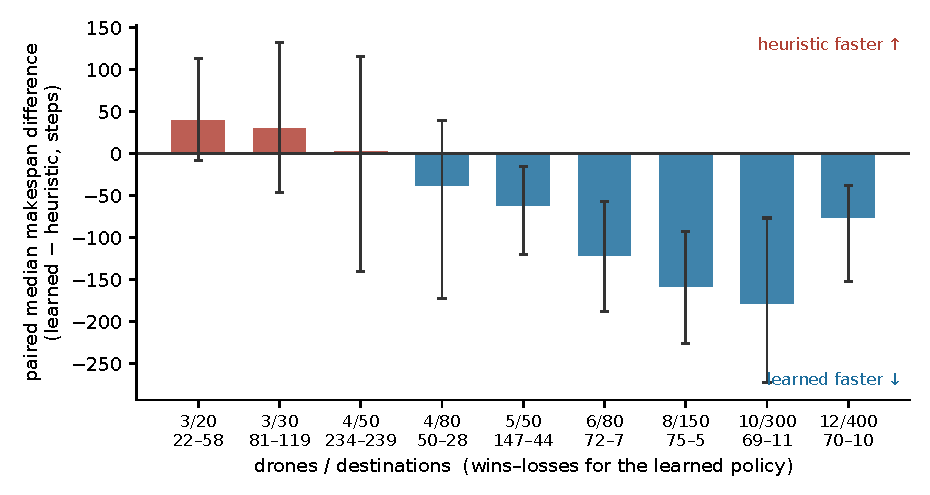
\includegraphics[width=\linewidth]{fig_regime_v5_26_10_17_15.pdf}
\caption{구성별 쌍별 중앙 makespan 차이(학습 $-$ 휴리스틱). 오차 막대는 쌍별 차이의 사분위 범위,
각 라벨 아래는 학습 정책의 승--패. 음수가 학습 정책에 유리하며 경계는 드론 4대에 있다.}
\label{fig:regime}
\end{figure}

그림~\ref{fig:cdf}는 세 주요 구성의 전체 분포다. 3대에서는 휴리스틱의 곡선이 왼쪽에 있고, 4대에서는
두 곡선이 겹치며, 5대에서는 학습 정책의 곡선이 왼쪽에 있고 더 일찍 완주에 닿는다.

\begin{figure*}[t]
\centering
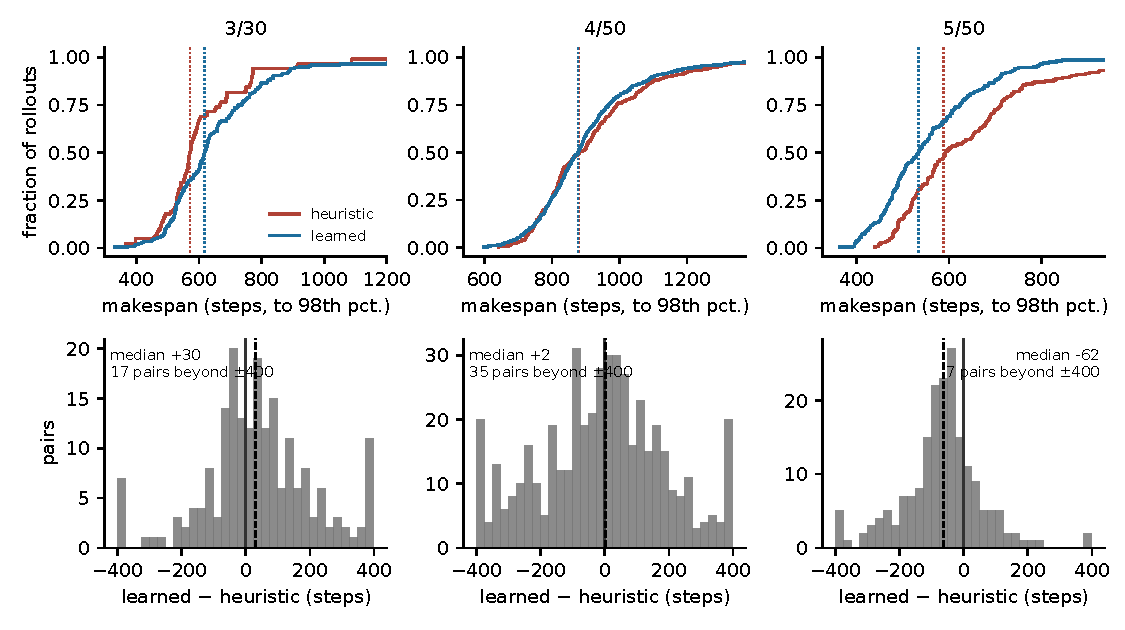
\includegraphics[width=\linewidth]{fig_cdf_v5_26_10_17_15.pdf}
\caption{위: $3/30$, $4/50$, $5/50$의 makespan 누적분포(점선은 중앙값, 축은 98 백분위에서
자름). 아래: 둘 다 완주한 인스턴스의 쌍별 차이 분포($\pm400$스텝에서 잘랐으며 잘린 쌍 수를
표기).}
\label{fig:cdf}
\end{figure*}

\paragraph{꼬리도 같은 방향으로 갈린다}
드론이 부족하면 학습 정책의 최악은 휴리스틱의 3--4배이고($3/30$에서 최댓값 5{,}395 대
1{,}447스텝), 넉넉하면 더 가볍다($5/50$에서 1{,}101 대 1{,}734, $10/300$에서 1{,}365 대 1{,}753).
튜닝 전 휴리스틱에 대한 표준 구성 480롤아웃에서 학습 정책은 1{,}500스텝을 다섯 번, 휴리스틱은 열네
번 넘었다.

\paragraph{기제}
두 제어기는 한 결정에서 다르다. $3/30$에서 휴리스틱은 평균 1.39대의 중계를 세우고 학습 정책은
0.78대를 세운다. 그 결과 학습 편대는 드론-스텝의 27\%를 투영에 막혀 정체하고 휴리스틱은 8\%다.
추론 시 학습 정책의 중계 배정만 휴리스틱의 것으로 덮으면 44스텝 격차 전부가 회복된다. 중계
\emph{대수}만 맞추면 중앙값은 14스텝만 회복되지만 꼬리는 사라진다(최댓값 4{,}904에서 1{,}083).
중계하는 드론의 정체가 중앙값을 만들고 대수가 꼬리를 만든다. 휴리스틱의 선택에 필요한 정보는
학습 정책의 관측에 있다. 2층 분류기가 41개 관측 특징으로 휴리스틱의 중계 배정을 85\% 정확도로
예측하고, 규칙 전체의 행동 복제는 중계 결정에서 95\%에 이른다. 드론이 넉넉하면 반대 일이
일어난다. 휴리스틱은 기하가 더 이상 요구하지 않는 사슬을 계속 세우는 반면, 학습 정책은 여유를
활용하고 표본 추론으로 결정론적 규칙이 반복하는 정체를 빠져나간다. 휴리스틱이 몇 건의 완주를 잃는
곳도 여기다.

\paragraph{드론 부족 영역의 열세가 정책 쪽 처방에 저항하는 이유}
\label{sec:negative}
표~\ref{tab:negative}는 드론이 부족할 때 학습 정책이 휴리스틱처럼 중계하게 만들려는 열 가지
개입이다. 각각 같은 조리법으로 시드 넷 또는 둘을 학습하고 같은 쌍별 규약으로 평가했다. 어느 것도
$3/30$ 중앙값을 개선하지 못했고 여럿은 학습 정책이 이기는 구성을 해쳤다. 패턴이 시사적이다. 중계에
보상을 더하면 수단이 목적이 된다. 정책이 중계 자체를 위해 중계하고 $5/50$이 $-54$에서 $+60$으로
뒤집힌다. 드론별 크레딧으로 가는 길은 각기 다른 이유로 막힌다. 결합 행동 critic은 목표값에 표본된
동료 행동의 분산을 물려받고, 단조 혼합망은 가중치가 자유로우면 발산하고 하한을 두면 평균으로
무너지며, 순차 단일 에이전트 재정식화는 분해를 없애지만 수축이 없는 무할인 크레딧 사슬을 남긴다.
규칙의 행동 복제로 정책을 초기화하면(중계 정확도 95\%) 400 에피소드 안에 지워진다. actor가
갱신되기 시작하면 50 에피소드 안에 중계 사용이 무작위 초기화 정책의 수준으로 떨어져 머문다. 병목
목적지의 추정 도달 시각에 대한 벌점은 정책이 최댓값이 아니라 \emph{평균}을 줄이게 만든다. 이
정책 구조와 목적함수 안에서 중계 부족은 크레딧·정보·초기화의 인공물이 아니라 학습기의
고정점이라고 결론짓는다.

\begin{table*}[t]
\centering
\caption{드론 부족 영역의 열세를 제거하지 못한 개입들. 휴리스틱 대비 쌍별 중앙값(양수가 느림),
제안 조리법이 기준 행. 이 실행들은 튜닝 전 탈출 파라미터($k_{\mathrm{stall}}=60$,
$h_{\mathrm{hold}}=40$)의 휴리스틱에 대해 평가되었으므로 이 표의 기준 행과는 비교 가능하지만
튜닝된 휴리스틱을 쓴 표~\ref{tab:paired}와 수치가 같지는 않다.}
\label{tab:negative}
\small
\begin{tabular}{lrrrl}
\toprule
개입 & $3/30$ & $5/50$ & $4/50$ & 실패 기제 \\
\midrule
제안 조리법 (기준) & $+40$ & $-54$ & $+0$ & --- \\
중계 가중 규칙 정규화 & $+54$, $+56$ & $-44$, $-19$ & $+41$, $+54$ & 중계 특화 정규화는 해로움 \\
드론별 중계 크레딧 & $+36$ ~ $+82$ & $+60$ ~ $+106$ & $+39$ ~ $+131$ & 중계가 목적이 됨 \\
$3/30$ 기준 체크포인트 선택 (8시드) & $+58$ & $-42$ & $+10$ & 표준 구성만 개선 \\
제로섬 크레딧 재분배 & $+91$, $+126$ & $+98$, $+172$ & $+146$, $+180$ & 같은 기제, 더 큼 \\
결합 행동 critic & $+89$ & $-27$ & $+58$ & 표본된 동료 행동의 목표값 분산 \\
가까운 드론부터 결정 & $+46$, $+100$ & $-43$, $-38$ & $+4$, $+106$ & 순서는 원인이 아님 \\
정체 시 재결정 (학습) & $+82$, $+95$ & $-38$, $-34$ & $+17$, $+55$ & 불규칙한 옵션 길이 \\
단조 혼합 critic & $+145$ & $+5$ & $+139$ & 발산 방지와 크레딧이 한 축 \\
순차 단일 에이전트 크레딧 & $+142$ & $+17$ & $+116$ & 결정 안에 수축 없음 \\
행동 복제 초기화 & $+42$ ~ $+69$ & $-42$ ~ $-20$ & $-4$ ~ $+40$ & 400 에피소드 안에 지워짐 \\
병목 도달 시각 벌점 & $+105$ & $-8$ & $+81$ & 최댓값이 아닌 평균을 줄임 \\
\bottomrule
\end{tabular}
\end{table*}

\paragraph{연결성 강제 모형에 대한 민감도}
\label{sec:sensitivity}
\ref{sec:projection}절의 투영은 막힌 변위를 같은 방향으로 축소하므로 사슬을 당기는 드론은 사실상
멈춘다. 목표 위치를 구속하는 이웃 주변 통신 원판의 가장 가까운 점으로 당기는 대안을 구현했다.
바깥 방향 성분만 제거하고 접선 성분은 남기므로 드론이 일정 거리를 유지한 채 돌 수 있다. 각 비교에서
두 제어기는 같은 투영을 쓰고 연결성은 여전히 위반되지 않는다. 이 측정은
\ref{sec:rq4-heuristic}절의 휴리스틱 튜닝 이전에 두 투영 모두 $k_{\mathrm{stall}}=60$,
$h_{\mathrm{hold}}=40$으로 한 것이라 내부적으로 일관된다. 같은 학습 가중치를 재학습 없이 접선 보존
투영에서 평가하면 $3/30$ 열세가 $+40$에서 $+21$로 줄고, 네 시드를 재학습하면 $+15$에서 $+48$(평균
$+28$)이 되며 학습 편대의 정체율은 0.27에서 0.17--0.22로 내려간다. 완주는 여전히 100\%다.
휴리스틱은 3대에서는 거의 얻지 못하지만(중앙값 570에서 571) 4대에서는 학습 정책보다 더 얻어(866에서
812, 학습은 879에서 850) 표준 구성의 동률이 휴리스틱 쪽 $+26$으로 바뀐다. 따라서 같은 방향 투영을
기본 모형으로 유지하고 이것을 민감도 결과로 보고한다. 3대 열세의 약 절반은 학습기가 아니라 제약을
강제하는 방식의 성질이다.

\paragraph{통신 반경}
두 제어기를 재학습 없이 $R = 250$\,m와 $R = 350$\,m에서 돌렸다(표~\ref{tab:range},
그림~\ref{fig:range}). 학습 정책은 거리를 $R$로 정규화하고 인스턴스 생성기는 도달 영역 $0.9NR$을
$R$에 맞춰 조정하므로 두 제어기는 각 반경에서 같은 인스턴스를 본다. 완주는 전이된다. 학습 정책은 두
반경 모두에서 모든 인스턴스를 완주하고, 휴리스틱은 짧은 반경의 $5/50$에서 200건 중 18건을 잃는다.
속도에는 두 효과가 나타난다. 첫째는 편대 크기에서 본 영역 이동이다. $R=250$\,m에서는 목적지에 더
많은 홉이 필요해 편대가 사실상 부족해지고 모든 구성이 휴리스틱 쪽으로 움직인다($3/30$ $+77$,
$4/50$ $+68$, $5/50$의 우위는 $-16$, $p=0.33$으로 동률까지 줄어든다). $R=350$\,m에서는 편대가 사실상
넉넉해져 학습 정책이 4대에서 이미 빠르다($4/50$ $-40$). 둘째는 학습 반경 효과다. $3/30$과 $5/50$에서
학습 정책의 격차는 학습한 반경에서 가장 좋고 양쪽에서 나빠진다(300\,m의 $+30$ 대 $+77$과 $+52$,
$-62$ 대 $-16$과 $-42$). $R$ 정규화는 완주를 전이시키지만 속도까지 온전히 전이시키지는 않는다.
따라서 영역 변수는 편대 크기만이 아니라 사슬 수요, 즉 목적지가 필요로 하는 홉 수 대 공급할 수 있는
드론 수이며, 학습 반경에서 먼 반경의 배치는 재학습하거나 적어도 경계를 재평가해야 한다.

\begin{figure}[t]
\centering
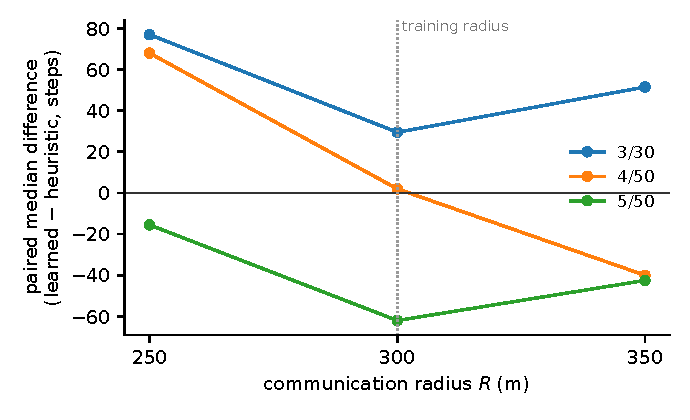
\includegraphics[width=\linewidth]{fig_range_v5_26_10_17_15.pdf}
\caption{재학습 없는 통신 반경별 쌍별 중앙 차이(학습 반경 300\,m, 점선). 짧은 반경은 모든 구성을
휴리스틱 쪽으로 옮기고, 긴 반경은 $4/50$에서 학습 정책을 돕지만 $3/30$과 $5/50$에서는 학습 반경의
격차를 넘지 못한다.}
\label{fig:range}
\end{figure}

\begin{table*}[t]
\centering
\caption{재학습 없는 다른 통신 반경으로의 전이. 셀은 완주(휴리스틱/학습)와 쌍별 중앙 차이(승--패,
$p$). $R=300$\,m가 학습 반경.}
\label{tab:range}
\small
\begin{tabular}{lrrr}
\toprule
$N/M$ & $R=250$\,m & $R=300$\,m & $R=350$\,m \\
\midrule
3/30 & 200/200 \,/\, $+77$ (45--154, $<10^{-4}$) & 200/200 \,/\, $+30$ (81--119, 3.4e-04) & 200/200 \,/\, $+52$ (58--141, $<10^{-4}$) \\
4/50 & 118/120 \,/\, $+68$ (40--77, $<10^{-4}$) & 473/480 \,/\, $+2$ (234--239, 0.521) & 119/120 \,/\, $-40$ (77--42, 1.1e-04) \\
5/50 & 182/200 \,/\, $-16$ (99--83, 0.327) & 191/200 \,/\, $-62$ (147--44, $<10^{-4}$) & 200/200 \,/\, $-42$ (152--46, $<10^{-4}$) \\
\bottomrule
\end{tabular}%

\end{table*}

\subsection{RQ4: 구성 요소는 필수적인가}
\label{sec:rq4}

\paragraph{휴리스틱}
\label{sec:rq4-heuristic}
표~\ref{tab:heur-ablation}은 $k_{\mathrm{stall}} \in \{30,60,90,120\}$,
$h_{\mathrm{hold}} \in \{20,40,80\}$, 두 탈출 모드, 그리고 탈출 없음을 $3/30$, $4/50$, $5/50$에서
각 40 튜닝 시드로 격자 탐색한 것이다. 설정은 완주 합 우선, 중앙 makespan 합 차선으로 순위를
매겼고 이 기준은 측정 전에 정했다. 탈출 장치는 필수다. 없으면 규칙은 표준 인스턴스 40건 중 26건을
완주한다. 시점보다 모드가 더 중요하다. 선두 교대 설정은 모두 120건 중 117--120건을 완주하는 반면
후퇴 설정은 100--117건을 완주하는데, 사슬을 느슨하게 해도 정체를 만든 배정이 바뀌지 않기 때문이다.
선두 교대 안에서는 세 구성 합산 중앙값이 최대 40스텝 차이로 40인스턴스의 잡음 안에 있다. 선택된
설정($k_{\mathrm{stall}}=120$, $h_{\mathrm{hold}}=20$)은 120건 전부를 완주한 유일한 설정이면서
중앙값 합도 가장 낮다. 적응적 중계 대수도 필수다. 한 대나 두 대로 고정하면 0--65\%를 완주한다
(표~\ref{tab:completion}).

\begin{table*}[t]
\centering
\caption{평가 시드와 분리된 튜닝 시드(구성당 40 인스턴스)에서의 휴리스틱 절제. 셀은 완주
인스턴스 수와 완주 인스턴스의 중앙 makespan, 마지막 열은 세 구성 완주 합.}
\label{tab:heur-ablation}
\small
\begin{tabular}{llrrrr}
\toprule
방식 & $k_{\mathrm{stall}}$ / $h_{\mathrm{hold}}$ & $3/30$ & $4/50$ & $5/50$ & 완주 합 \\
\midrule
없음 & --- & 39/40 \,/\, 559 (0.228) & 25/40 \,/\, 817 (0.258) & 38/40 \,/\, 602 (0.093) & 102/120 \\
선두 교대 & 30 / 20 & 40/40 \,/\, 557 (0.121) & 39/40 \,/\, 853 (0.130) & 40/40 \,/\, 625 (0.928) & 119/120 \\
선두 교대 & 30 / 40 & 40/40 \,/\, 562 (0.673) & 40/40 \,/\, 867 (0.775) & 40/40 \,/\, 606 (0.247) & 120/120 \\
선두 교대 & 30 / 80 & 40/40 \,/\, 567 (0.158) & 39/40 \,/\, 844 (0.754) & 39/40 \,/\, 614 (0.404) & 118/120 \\
선두 교대 & 60 / 20 & 40/40 \,/\, 557 (0.599) & 39/40 \,/\, 849 (0.780) & 40/40 \,/\, 600 (0.791) & 119/120 \\
선두 교대 & 60 / 40 & 40/40 \,/\, 554 (0.497) & 39/40 \,/\, 852 (0.807) & 40/40 \,/\, 625 (0.944) & 119/120 \\
선두 교대 & 60 / 80 & 40/40 \,/\, 556 (0.359) & 39/40 \,/\, 863 (0.788) & 39/40 \,/\, 632 (0.675) & 118/120 \\
선두 교대 & 90 / 20 & 40/40 \,/\, 566 (0.206) & 39/40 \,/\, 871 (0.908) & 40/40 \,/\, 599 (0.375) & 119/120 \\
선두 교대 & 90 / 40 & 40/40 \,/\, 559 (0.473) & 40/40 \,/\, 856 (0.674) & 37/40 \,/\, 634 (0.844) & 117/120 \\
선두 교대 & 90 / 80 & 40/40 \,/\, 563 (0.786) & 39/40 \,/\, 858 (0.149) & 39/40 \,/\, 629 (0.615) & 118/120 \\
\textbf{선두 교대} & \textbf{120 / 20} & 40/40 \,/\, 561 & 40/40 \,/\, 867 & 40/40 \,/\, 620 & \textbf{120/120} \\
선두 교대 & 120 / 40 & 40/40 \,/\, 557 (0.757) & 39/40 \,/\, 878 (0.685) & 40/40 \,/\, 624 (0.979) & 119/120 \\
선두 교대 & 120 / 80 & 40/40 \,/\, 562 (0.687) & 38/40 \,/\, 829 (0.546) & 39/40 \,/\, 626 (0.850) & 117/120 \\
후퇴 & 30 / 20 & 37/40 \,/\, 559 (0.350) & 35/40 \,/\, 836 (0.185) & 40/40 \,/\, 632 (0.528) & 112/120 \\
후퇴 & 30 / 40 & 39/40 \,/\, 556 (0.079) & 29/40 \,/\, 832 (0.284) & 39/40 \,/\, 621 (0.157) & 107/120 \\
후퇴 & 30 / 80 & 38/40 \,/\, 561 (0.754) & 26/40 \,/\, 804 (0.443) & 37/40 \,/\, 584 (0.368) & 101/120 \\
후퇴 & 60 / 20 & 39/40 \,/\, 556 (0.866) & 38/40 \,/\, 847 (0.215) & 38/40 \,/\, 603 (0.759) & 115/120 \\
후퇴 & 60 / 40 & 39/40 \,/\, 559 (0.875) & 39/40 \,/\, 823 (0.485) & 39/40 \,/\, 624 (0.459) & 117/120 \\
후퇴 & 60 / 80 & 39/40 \,/\, 563 (0.991) & 26/40 \,/\, 795 (0.236) & 40/40 \,/\, 635 (0.490) & 105/120 \\
후퇴 & 90 / 20 & 39/40 \,/\, 566 (0.512) & 38/40 \,/\, 822 (0.058) & 40/40 \,/\, 642 (0.773) & 117/120 \\
후퇴 & 90 / 40 & 39/40 \,/\, 566 (0.180) & 39/40 \,/\, 852 (0.634) & 39/40 \,/\, 618 (0.615) & 117/120 \\
후퇴 & 90 / 80 & 39/40 \,/\, 562 (0.665) & 36/40 \,/\, 830 (0.578) & 37/40 \,/\, 598 (0.354) & 112/120 \\
후퇴 & 120 / 20 & 39/40 \,/\, 556 (0.645) & 37/40 \,/\, 863 (0.327) & 38/40 \,/\, 614 (0.460) & 114/120 \\
후퇴 & 120 / 40 & 39/40 \,/\, 560 (0.757) & 37/40 \,/\, 831 (0.451) & 38/40 \,/\, 628 (0.602) & 114/120 \\
후퇴 & 120 / 80 & 39/40 \,/\, 561 (0.191) & 38/40 \,/\, 854 (0.815) & 37/40 \,/\, 627 (0.308) & 114/120 \\
\bottomrule
\end{tabular}%

\end{table*}

\paragraph{학습 정책}
표~\ref{tab:ablation}은 요소를 하나씩 빼고 시드 둘을 재학습해 세 주요 구성에서 평가한 것으로, 값은
제안 조리법 대비 makespan 차이다. 같은 조리법을 네 번 독립 학습하면 표준 구성에서 919에서
979스텝까지 흩어지므로 시드 2개 평균은 70--80스텝을 넘을 때만 의미가 있다. 규칙 정규화와 구성
무작위화는 필수이고, 엔트로피 감쇠는 표준 구성에서 가장 큰 단일 기여이며, 자기회귀 결정은 4대
이상에서 돕고, 잔여 벌점은 중립이다. 초기 버전에서 표준 구성만으로 학습한 고정 크기 MLP 인코더의
상위 정책은 표준 인스턴스의 38\%를 완주했고 다른 편대 크기에서는 아예 돌릴 수 없었다.

\begin{table}[t]
\centering
\caption{학습 정책의 절제: 완주 에피소드에서 제안 조리법 대비 makespan 차이, 시드 2개. 양수는 뺀
요소가 필요했다는 뜻. 70--80스텝 아래의 차이는 시드 분산 안이다.}
\label{tab:ablation}
\small
\begin{tabular}{lrrr}
\toprule
제거한 요소 & $4/50$ & $3/30$ & $5/50$ \\
\midrule
규칙 정규화 & $+320$ & $+408$ & $+92$ \\
구성 무작위화 & $-44$ & $+646$ & $+68$ \\
엔트로피 목표 감쇠 & $+128$ & $+19$ & $+61$ \\
자기회귀 결정 & $+94$ & $-46$ & $+33$ \\
잔여 벌점 & $-28$ & $-37$ & $+8$ \\
\bottomrule
\end{tabular}
\end{table}

\subsection{추론 비용}
\label{sec:cost}

표~\ref{tab:latency}는 CPU에서 상위 결정 1회의 지연이다. 휴리스틱은 0.05--0.12\,ms, 학습 정책은
자기회귀 없이 1.3--2.5\,ms, 자기회귀로 2.7--7.4\,ms이며 드론마다 순차 네트워크 호출이라 편대에
선형으로 커진다. 900스텝 에피소드에서 학습 정책의 누적 결정 시간은 0.16\,s다. 격자 MILP는 목적지
4--10곳 인스턴스에서 600--5{,}400초가 걸리고 10곳에서는 계획을 내지 못한다.

\begin{table*}[t]
\centering
\caption{상위 결정 1회의 지연(밀리초, CPU)과 900스텝 에피소드의 누적 결정 시간.}
\label{tab:latency}
\small
\begin{tabular}{lrrrrr}
\toprule
제어기 & $N=3$ & $N=4$ & $N=6$ & $N=8$ & 900스텝 \\
\midrule
기하 규칙 + 탈출 & 0.05 & 0.08 & 0.10 & 0.12 & 0.003\,s \\
학습, 독립 결정 & 1.27 & 1.52 & 1.94 & 2.45 & 0.069\,s \\
학습, 자기회귀 (제안) & 2.70 & 3.52 & 5.32 & 7.35 & 0.158\,s \\
\bottomrule
\end{tabular}
\end{table*}

% =====================================================================================
\section{논의}
\label{sec:discussion}

\paragraph{배치}
두 제어기는 상보적이고 경계가 뚜렷하므로 운영자는 편대 크기로 고를 수 있다. 드론 3대면 휴리스틱,
5대 이상이면 더 빠르고 더 신뢰할 수 있는 학습 정책이며, 4대에서는 둘이 동률이고 학습 정책이 더 많이
완주한다. 둘 다 밀리초에 결정하고 둘 다 구조적으로 편대의 연결을 지킨다.

\paragraph{음성 결과의 의미}
학습기의 크레딧·정보·초기화·보상을 바꾸는 열 개입이 드론 부족 영역의 열세를 그대로 두었고, 환경의
강제 모형을 바꾸자 절반이 사라졌다. 따라서 이 열세는 더 학습하거나 더 나은 critic으로 고칠 결함이
아니라, 이 목적함수 아래 학습기의 고정점과 제약의 기하 사이의 상호작용으로 이해하는 것이 맞다.
실무자에게 실행 가능한 결론은 위의 것 하나다. 영역에 따라 제어기를 고르라.

\paragraph{한계}
학습 정책은 하나의 통신 반경에서 학습했다. 250과 350\,m로 완주는 전이되지만 휴리스틱 대비 속도
순위는 반경에 따라 바뀌며(\ref{sec:rq3}절), 그 밖의 반경은 시험하지 않았다. 환경은 평면이고
바람·배터리·충돌을 무시하며 원판 통신 모형을 쓴다. 실제 링크는 원판이 아니다. MILP 참조는 최적성 갭이
남은 격자 제한이지 정확한 최적값이 아니다. 휴리스틱의 참신성은 사슬 기하 자체보다 탈출 장치와
적응적 중계 대수에 있다.

\paragraph{방법론적 주석}
결론에 중요했던 세 실천이 있다. 완주 에피소드 평균은 포기하는 제어기에 유리하므로 비교는 쌍별이어야
한다. 40롤아웃은 꼬리에 관한 주장을 뒷받침하지 못하며, 우리 자신의 중간 결론 여럿이 표본이 커지자
뒤집혔다. 그리고 최종 판정과 다른 지표를 쓰는 사전 점검은 최종 판정이 기각할 개입을 통과시킨다.

% =====================================================================================
\section{결론}
\label{sec:conclusion}

연결성 제약 드론 배송을 위한 두 제어기, 교착 탈출을 갖춘 기하 사슬 중계 휴리스틱과 편대 크기 불변
학습 정책을 제안했다. 둘 다 매 스텝 편대를 연결 상태로 유지하는 투영을 통해 행동한다. 드론 3--10대
편대의 쌍별 규약에서 학습 정책은 모든 인스턴스를 완주하고 4대를 넘는 드론이 있으면 38--178스텝
빠르며, 3대에서는 휴리스틱이 30--39스텝 빠르다. 드론 부족 영역의 열세는 어느 드론이 중계할지라는
한 결정이며, 열 가지 정책 쪽 개입에 저항하고 강제 모형을 바꾸면 절반으로 준다. 두 제어기는 목적지
10곳에서 계획을 내지 못하는 격자 정확 최적화보다 세 자릿수 빠르다. 자연스러운 다음 단계는 출력이
드론별 옵션 집합이 아니라 팀 배정인 정책으로, 중계 드론의 정체를 critic이 직접 평가할 수 있는
좌표로 만드는 것이다.

\section*{감사의 글}
\pending{추가 예정.}

\section*{데이터와 코드}
코드, 학습 가중치, 인스턴스 생성기, 쌍별 비교 기록은
\url{https://github.com/koptimizer/relay_drone_network}에서 받을 수 있다.

\bibliographystyle{elsarticle-num}
\bibliography{paper_v5_26_10_17_15}

\end{document}
